\section{Methods}\label{sec:methods}

Loosely following \citet{smith1979existence} we formulate the traffic assignment problem as follows.
Let $G=(N,L)$ represent a finite directed graph with $N$ denoting the set of nodes with $n$ members and $L$ the set of links with $m$ members.
We denote each link as $a_i\in L$ for $i=1,\cdots,m$ and the traffic flow across each link as $x_i$ for $i=1,\cdots,m$.
We collect the link flows in a vector $\mathbf{x}=(x_1,\cdots, x_m)\in\mathbb{R}_+^m$. 
Where $\mathbb{R}_+^m$ denotes the non-negative orthant of $\mathbb{R}^m$.
Similarly we define a vector of link capacities, $\mathbf{c}=(c_1, \cdots, c_m)\in \mathbb{R}_+^m$.

Let $Q\subseteq N\times N$ denote the set of origin-destination pairs on the network with $|Q| = d$.
Denote by $q_i$ the travel demand between each origin-destination pair for $i=1,\cdots,d$.
We collect the demand as a vector $\mathbf{q}=(q_1, \cdots, q_d)\in\mathbb{R}_+^d$. 
The goal of the traffic assignment problem is to allocate the volume of travel demand to links in the network such that all travellers reach their destination and Wardrop's first condition is met.

Intuitively, however, the choice faced by drivers is in terms of paths through the network, not specific links.
A \textit{path} in the network retains its graph-theoretic definition: an ordered sequence of directed links in the network which connect two nodes in the graph. 
We may enumerate all (directed) paths in the network as a set $P$ and let $p=|P|$
A \textit{path flow} is a vector $\mathbf{F}\in \mathbb{R}^p_+$ which represents the volume of traffic along each path in the network.
A path flow is \textit{demand feasible} if the total volume of traffic on all paths between each origin destination pair is equal to the travel demand between that origin destination pair.
In other words, if there are 10 vehicles trying to get from point A to point B and there are two paths connecting A and B, the sum of the volumes on the two paths had better be equal to 10.
Define $M \in \{0, 1\}^{d\times p}$ to be a binary matrix representing the trip-path incidence relation: $M_{ij} = 1$ if the $j$-th path in $P$ connects the origin-destination pair $q_i$ and equals $0$ otherwise.
With this definition, a path flow $\mathbf{F}$ is demand feasible if $M\mathbf{F}=\mathbf{q}$.

A path flow vector induces traffic volume on each link.
We can make explicit this relation by defining the \textit{link-path} incidence matrix.
Let $D\in \{0, 1\}^{p\times m}$ be a binary matrix representing the link-path incidence relation: $D_{ij}=1$ if link $a_j$ is on the $i$-th path of $P$ and equals $0$ otherwise. 
The volume of traffic on each link is given by $\mathbf{x}\in \mathbb{R}_+^m$ and referred to as the \textit{link flow}.
A link flow $\mathbf{x}$ corresponds to a path flow $\mathbf{F}$ if $\mathbf{x} = D^T\mathbf{F}$.
A link flow is said to be \textit{demand-feasible} if is corresponds to a demand-feasible path-flow.
A link flow $\mathbf{x}\in \mathbb{R}_+^m$ is said to be \textit{supply-feasible} if its value on each link does not exceed the capacity of the link: $x_i \leq c_i$ for all $i=1\cdots m$.

We may now represent the set of demand-feasible and supply-feasible link flows.

\begin{align}
    \Omega_d &= \{\mathbf{x} \in \mathbb{R}_+^m \mid \exists \mathbf{F} \in \mathbb{R}^p_+ M (\mathbf{F}= \mathbf{q} \land D^T\mathbf{F} = \mathbf{x})\} \label{eqn:demand-feasible-link-flow}\\
    \Omega_s &= \{\mathbf{x} \in \mathbb{R}_+^m \mid \mathbf{x} \preceq \mathbf{c} \} \label{eqn:supply-feasible-link-flow}\\
    \Omega &= \Omega_d \cap \Omega_s
\end{align}

Where we use $\preceq$ to denote element-wise inequality.
To simplify the notation for the rest of this paper we will use $\Omega$ to refer to the supply and demand feasible set $\Omega_d\cap \Omega_s$.

Finally, we introduce the link cost function $\mathbf{t}: \Omega_s \to \mathbb{R}_+^m$ which reports the travel cost of each link as a function of the link flows.
We denote the cost of a single link $a_i$ as $t_i(\mathbf{x})$.

The user equilibrium condition introduced by \citet{wardrop1952some} can be expressed succinctly as a \textit{variational inequality} \citep{smith1979existence,dafermos1980traffic,nagurney2009netecon}.
We motivate the variational inequality formulation by returning to the decision process outlined in \cref{sec:motivating-example}.
Using our notation let $\mathbf{x}^*$ denote yesterday's link flows and let $\mathbf{x}$ denote today's link flows which have yet to be decided.
The link costs induced by yesterday's flow is therefore given by $\mathbf{t}(\mathbf{x}^*)$.
This cost may be regarded as fixed because it was induced by link flows from yesterday.
In order for yesterday's link flows to be at equilibrium, there can be no alternative feasible link flow which reduces the total cost based on yesterday's costs.
Mathematically, yesterday's total cost is given by $\mathbf{t}(\mathbf{x}^*)\mathbf{x}^*$ and the cost of today's potential route choice $\mathbf{x}$ based on yesterday's costs is given by $\mathbf{t}(\mathbf{x}^*)\mathbf{x}$. 
So $\mathbf{x}^*$ is at equilibrium if and only if $\mathbf{t}(\mathbf{x}^*)\mathbf{x}^* \leq \mathbf{t}(\mathbf{x}^*)\mathbf{x}$.

We therefore say that $\mathbf{x^*}\in\Omega$ is an equilibrium link flow if \eqref{eqn:ui-vi} holds.

\begin{theorem}[Variational Inequality Formulation]
    \label{thm:ui-vi}
    A link flow pattern $\mathbf{x}^* \in \Omega$ is a traffic network equilibrium link flow if and only if it satisfies the following variational inequality problem:
    \begin{align}
        \mathbf{t}(\mathbf{x^*})(\mathbf{x}- \mathbf{x^*}) &\geq 0,\ \text{for all}\ \mathbf{x} \in \Omega \label{eqn:ui-vi}
    \end{align}
\end{theorem}

\begin{theorem}[Existence]
\label{thm:existence}
    There exists an equilibrium link flow $\mathbf{x}^* \in \Omega_d \cap \Omega_s$ if the following conditions are met.
    \begin{enumerate}
        \item The link cost function $\mathbf{t}: \Omega_s \to \mathbb{R}_+^m$ is continuous.\label{exists-condition:link-cost-continuous}
        \item The demand-feasible set of link flows $\Omega_d$ is closed and convex.\label{exists-condtions:demand-convex}
        \item Every demand-feasible link flow is also supply feasible: $\Omega_d \subseteq \Omega_s$. \label{exists-condtion:demand-supply-feasible}
    \end{enumerate}
\end{theorem}

The proof of \cref{thm:existence} is given in \citet{smith1979existence}.
Of the conditions on existence that \cref{thm:existence} requires, only one is non-trivial.
Condition \ref{exists-condition:link-cost-continuous} is very mild and not unreasonable in practice.
The demand-feasible set as defined in \eqref{eqn:demand-feasible-link-flow} meets condition \ref{exists-condtions:demand-convex} since it is defined by a set of linear constraints.
Condition \ref{exists-condtion:demand-supply-feasible}, as Smith notes, is rather strong.
This condition arises from the use of the Brouwer fixed-point theorem, which states that every continuous mapping from a non-empty convex and compact set into itself has a fixed point.
In short, the proof leverages a continuous mapping  $T: \Omega_d\cap \Omega_s \to \Omega_d$ so in order to apply the theorem, $\Omega_d$ needs to be a subset of $\Omega_s$.
Besides, $\mathbf{t}$ is not defined outside of $\Omega_s$.
There are alternate existence theorems that relax this constraint but for simplicity we will use this one. 

There are also uniqueness conditions which we do not consider in this project.
Uniqueness is used to show that an algorithm that finds \textit{an} equilibrium has found the right one. 
In this project we do not compute the equilibrium state explicitly, we do not care much if there is more than one equilibrium. For the rest of this paper we \textbf{do not} assume uniqueness of the equilibrium state.


The network design problem additionally introduces a network control system which implicitly modifies the network cost.
A classical example of a network design problem is presented in \citet{sheffi1983optimal}.
The timing of traffic signals in the network is controlled with the intent of minimizing the total delay in the network.
What makes this problem difficult is that changes to the signal timing changes the travel costs of the links which changes the equilibrium traffic flow which determines the total delay.

Let $Y\subseteq \mathbb{R}^k$ denote the domain of the control parameters. The link cost $\mathbf{t}$ now additionally depends on the control parameters.
Let $g:\mathbb{R}^k\times \mathbb{R}^m\to \mathbb{R}$ be a network performance function which depends jointly on the state of the network and on the control parameters.
In the example given by \citet{sheffi1983optimal}, this would simply be the total delay in the network.
We express the network design problem as a mathematical program with equilibrium constraints in \eqref{eqn:ndp-mpec}.

\begin{subequations}
\begin{align}
    \min_{\mathbf{y}\in Y}\ & g(\mathbf{y}, \mathbf{x^*})\\
    \st 
        & \mathbf{x^*} \in \Omega\\
        &  \mathbf{t}(\mathbf{y}, \mathbf{x^*})(\mathbf{x}- \mathbf{x^*}) \geq 0,\ \text{for all}\ \mathbf{x} \in \Omega
\end{align}\label{eqn:ndp-mpec}
\end{subequations}

\subsection{The Braess Network}

As a croncrete network we introduce the Braess Network as described by \citet{Murchland1970} in \cref{fig:braess-network}.

\begin{figure}[!ht]
    \centering
    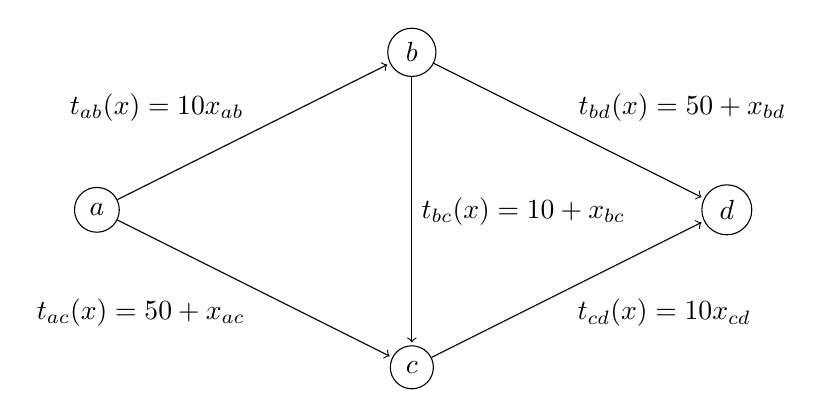
\begin{tikzpicture}[vertex/.style={circle, draw}]
        \node[style=vertex] (a) at (-4, 0)  {$a$};
        \node[style=vertex] (b) at (0, 2)  {$b$};
        \node[style=vertex] (c) at (0, -2) {$c$};
        \node[style=vertex] (d) at (4, 0)  {$d$};
        
        \draw[every loop]
            (a) edge node[above left] {$t_{ab}(x)=10 x_{ab}$} (b)
            (a) edge node[below left] {$t_{ac}(x)=50 + x_{ac}$} (c)
            (b) edge node[above right] {$t_{bd}(x)=50 + x_{bd}$} (d)
            (c) edge node[below right] {$t_{cd}(x)=10 x_{cd}$} (d)
            (b) edge node[right] {$t_{bc}(x)=10+x_{bc}$} (c)
        ;
    \end{tikzpicture}
    \caption{The Braess network. Each link is labeled with the link cost function.}
    \label{fig:braess-network}
\end{figure}

On this network there is only one origin-destination pair: $(a, d)$.
Let $q=6$ denote the travel demand from $a$ to $d$.
Further, we assume that the road network has sufficient capacity for all vehicles.
In particular, we may take capacity equal to $q$ for each link. 
There are three paths between $a$ and $d$ on this network: $(a, b, d)$, $(a,c,d)$, and $(a, b, c, d)$.
We will refer to these three paths as \textit{upper}, \textit{lower}, and \textit{zig-zag} paths respectively.

\citet{Murchland1970} states the equilibrium is achieved when each of the three paths is used by two vehicles each.
Immediately we see that such a path flow is demand-feasible since the path flows sum to equal the demand.
To convince ourselves that such a path flow is indeed at equilibrium, we can apply Wardrop's first principle directly: all used paths should have equal travel cost.
First, let us compute the corresponding link flow.
We could construct the link-path incidence matrix, but for this small example it is easier to simply enumerate in \cref{tab:braess:equilibrium-costs}.
The link cost is computed by applying the link cost function associated with each link in \cref{fig:braess-network}.

\begin{table}[!ht]
\centering
\caption{Link flow and link costs}\label{tab:braess:equilibrium-costs}
\begin{tabular}{@{}l|lll|ll@{}}
\toprule
Link & Upper & Lower & Zig-zag & Link flow & Link cost \\ \midrule
ab   & 2     & 0     & 2       & 4         & 40        \\
bd   & 2     & 0     & 0       & 2         & 52        \\
ac   & 0     & 2     & 0       & 2         & 52        \\
cd   & 0     & 2     & 2       & 4         & 40        \\
bc   & 0     & 0     & 2       & 2         & 12        \\ \bottomrule
\end{tabular}
\end{table}

We can compute the path costs by simply adding up the costs on each link of the path.
The upper path is composed of ab and bd, the lower by ac and cd, and the zig-zag by ab, bc, and cd.
The path costs are therefore $40+52=92$ for the upper path, $52+40=92$ for the lower path, and $40+12+40=92$ for the zig-zag path.
We observe that all paths that are used have equal cost.
Therefore Wardrop's first condition is met and this link flow is an equilibrium.

Alternatively we use this example to understand why Wardrop's first condition is equivalent to the condition that no driver has a less costly alternative route.
When all paths between their origin and destination cost the same, the driver had no incentive to switch routes.

Additionally, we can use the VI path flow formulation at this equilibrium and show that the following holds for all feasible path flows.

\begin{align*}
    \mathbf{T}(\mathbf{f}^*)\mathbf{f} - \mathbf{T}(\mathbf{f}^*)\mathbf{f}^* &\geq 0\\
    92\cdot f_{\text{upper}} + 92\cdot f_{\text{lower}} + 92 \cdot f_{\text{zig-zag}} - (92\cdot 2 + 92\cdot 2 + 92\cdot 2) &\geq 0\\
    f_{\text{upper}} + f_{\text{lower}} + f_{\text{zig-zag}} &\geq 6
\end{align*}

Recall that a path flow is feasible if the total volume over paths between and origin-destination pair is equal to the demand between that pair.
Therefore, $f_{\text{upper}} + f_{\text{lower}} + f_{\text{zig-zag}}=6$ for all feasible path flows and the inequality holds.\\


This particular network is notable because its equilibrium traffic flow is not its most efficient traffic assignment, giving rise to what is known as the ``Braess Paradox''.
Consider instead the demand-feasible path flow which puts three vehicles each on the upper and lower paths and none on the zig-zag path.
The link costs for this path flow are given in \cref{tab:braess:optimal-costs}.

\begin{table}[!ht]
\centering
\caption{Link flow and link costs}\label{tab:braess:optimal-costs}
\begin{tabular}{@{}l|lll|ll@{}}
\toprule
Link & Upper & Lower & Zig-zag & Link flow & Link cost \\ \midrule
ab   & 3     & 0     & 0       & 3         & 30        \\
bd   & 3     & 0     & 0       & 3         & 53        \\
ac   & 0     & 3     & 0       & 3         & 53        \\
cd   & 0     & 3     & 0       & 3         & 30        \\
bc   & 0     & 0     & 0       & 0         & 10        \\ \bottomrule
\end{tabular}
\end{table}

With this path flow, the travel costs on each of the used paths is 83.
This is less than the cost of the paths at equilibrium, meaning that this is globally more efficient.
However, this flow pattern is not an equilibrium because the unused zig-zag path has cost equal to 70 ($=30+10+30$), less than the cost of the used paths.
As a result, a single driver on the upper or lower path would be able to switch to the zig-zag path and save time.
This fact contradicts Wardrop's first condition.

As a VI in the path flow formulation we may find a path flow which does not satisfy the inequality.

\begin{align*}
    \mathbf{T}(\mathbf{f}^*)\mathbf{f} - \mathbf{T}(\mathbf{f}^*)\mathbf{f}^* &\geq 0\\
    83\cdot f_{\text{upper}} + 83\cdot f_{\text{lower}} + 70 \cdot f_{\text{zig-zag}} - (83\cdot 3 + 83\cdot 3 + 70\cdot 0) &\geq 0\\
    83\cdot f_{\text{upper}} + 83\cdot f_{\text{lower}} + 70 \cdot f_{\text{zig-zag}} \geq 83\cdot 6 
\end{align*}

In particular take $f_{\text{zig-zag}}=6$ (and no flow on either of the other two paths). Substituting this path flow into the inequality yields $70\cdot 6 \geq 83 \cdot 6$ which is false.



%This project will model this interaction between the network control system and the equilibrium traffic flow as a differential hybrid game.
%The central component of the model is the travel cost which will be expressed as a part of a differential equation to which the control system and vehicle fleet jointly provide input.
%The network performance function will serve as the \textit{terminal payoff} function.
%Concretely, this will involve the following steps,
%
%\begin{enumerate}
%    \item Formulate the network design problem on the Braess Network
%    \footnote{The Braess Network \citep{frank1981braess} is the smallest network to exhibit the Braess Paradox: in which \textit{removing} a link \textit{reduces} total congestion under user equilibrium traffic flow.
%    In other words, the user equilibrium flow on this network is provably not the system optimal flow.}
%    as a differential hybrid game where the ``angel'' role is played by the traffic control system and the ``demon'' role is played by the vehicle fleet.
%    To simplify matters we suppose that the traffic control system is able to charge a toll to vehicles for use of the roadway.
%    \item Introduce the network performance function as the \textit{terminal payoff}.
%    In this case the control system aims to reduce congestion in the network.
%    \item Prove that the traffic control system has a winning strategy to reduce total congestion.
%    \item Develop component-based verification for network at equilibrium analogous to \citet{DBLP:conf/itsc/MullerMP15}.
%\end{enumerate}